\section{MeshConvert}
\label{s:utilities:meshconvert}

\newcommand{\mc}{\texttt{MeshConvert}\xspace}
\newcommand{\gmsh}{\texttt{Gmsh}\xspace}

\mc is a utility bundled with \nekpp which has two purposes:
\begin{itemize}
  \item allow foreign mesh file formats to be converted into \nekpp's XML
  format;
  \item aide in the generation of high-order meshes through a series of supplied
  processing modules.
\end{itemize}

There is also some limited support for other output formats. We begin by running
through a basic example to show how a mesh can be converted from the widely-used
mesh-generator \gmsh to the XML file format.

\subsection{Exporting a mesh from \gmsh}

To demonstrate how \mc works, we will define a simple channel-like 3D geometry.
First, we must define the \gmsh geometry to be used. The \gmsh definition is
given below, and is visualised in figure~\ref{fig:util:mc:gmsh-example}.

\begin{lstlisting}[style=XmlStyle]
Point(1) = {-1, 0, 0, 1.0};
Point(2) = {-0.3, 0, 0, 1.0};
Line(3) = {1, 2};
s[] = Extrude {0, 0, 7} {
  Line{3}; Layers{5}; Recombine;
};
v[] = Extrude {{0, 0, 1}, {0, 0, 0}, Pi} {
  Surface{s[1]}; Layers{10}; Recombine;
};
\end{lstlisting}

Whilst a full tutorial on \gmsh is far beyond the scope of this document, note
the use of the \texttt{Recombine} argument. This allows us to generate a
structured hexahedral mesh; remove the first \texttt{Recombine} to generate a
prismatic mesh and both occurances to generate a tetrahedral mesh. Increasing
the \texttt{Layers} numbers refines the mesh in the radial and azimuthal
direction respectively.

\subsection{Defining physical surfaces and volumes}

\begin{figure}
  \begin{center}
    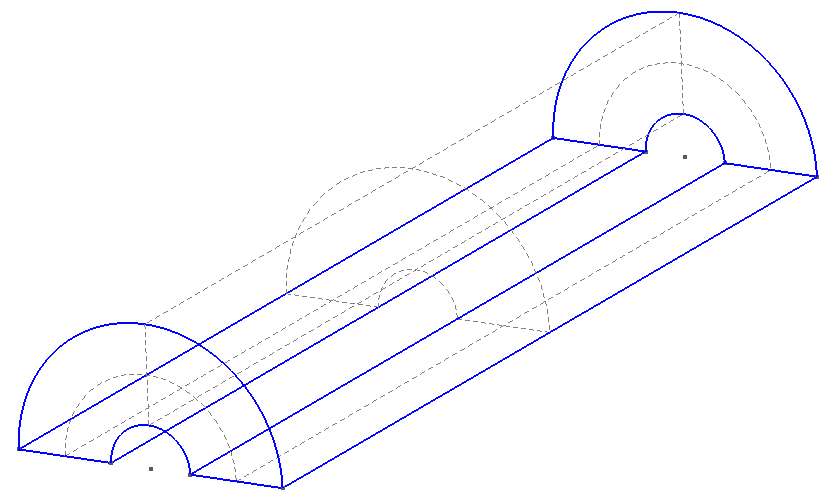
\includegraphics[width=0.4\textwidth]{utilities/Figures/mc-example-gmsh}
    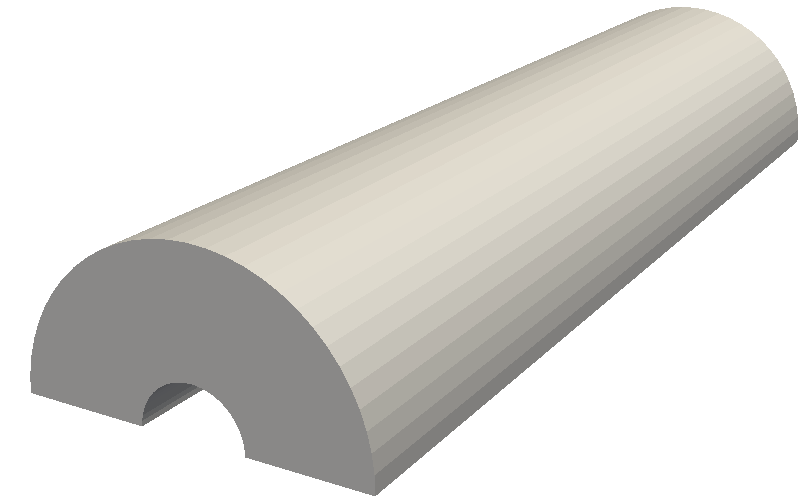
\includegraphics[width=0.4\textwidth]{utilities/Figures/mc-example-mesh}
  \end{center}
  \caption{Geometry definition in Gmsh (left) and resulting high-order mesh
    visualised in ParaView (right).}
  \label{fig:util:mc:gmsh-example}
\end{figure}

In order for us to use the mesh, we need to define the physical surfaces which
correspond to the inflow, outflow and walls so that we can set appropriate
boundary conditions. The numbering resulting from the extrusions in this case is
not straightforward. In the graphical interface, select \inlsh{Geometry >
  Physical Groups > Add > Surface}, and then hover over each of the surfaces
which are shown by the dashed gray lines. The numbering will be revealed in the
toolbar underneath the geometry as a ruled surface. In this case:
%
\begin{itemize}
\item \textbf{Walls:} surfaces 7, 8, 28, 29.
\item \textbf{Inflow:} surface 16.
\item \textbf{Outflow:} surface 24.
\end{itemize}
%
We also need to define the physical volumes, which can be done in a similar
fashion. For this example, there is only one volume having ID 1. Adding these
groups to the end of the \texttt{.geo} file is very straightforward:

\begin{lstlisting}[style=XmlStyle] 
Physical Volume(0) = {1};
Physical Surface(1)= {7,8,28,29};
Physical Surface(2) = {16};
Physical Surface(3) = {24};
\end{lstlisting}
Either choose the option \inlsh{File->Save Mesh} or, assuming this is saved in
a file named \inlsh{test.geo}, run the command 
\begin{lstlisting}[style=BashInputStyle]
gmsh -3 test.geo
\end{lstlisting}
which will produce the resulting MSH file \inlsh{test.msh}. One can generate a
high-order mesh by specifying the order on the command line, for example
\begin{lstlisting}[style=BashInputStyle] 
gmsh -3 -order 6 test.geo
\end{lstlisting}
will generate a sixth-order mesh. Note that you will need to use a current
version of \gmsh in order to do this, most likely from subversion.

\subsection{Converting the MSH to Nektar++ format}
Assuming that you have compiled \nekpp according to the compilation
instructions, run the command
%
\begin{lstlisting}[style=BashInputStyle]
MeshConvert test.msh test.xml
\end{lstlisting}
%
to generate the XML file. 
%
\begin{notebox}
  This file contains only the geometry definition (and a default
  \inltt{EXPANSIONS} definition). In order to use this mesh, a
  \inltt{CONDITIONS} section must be supplied detailing the solver and
  parameters to use.
\end{notebox}
%
To validate the mesh visually, we can use a utility such as Paraview or
VisIt. To do this, run the command
%
\begin{lstlisting}[style=BashInputStyle]
XmlToVtk test.xml
\end{lstlisting}
%
which generates an unstructured VTK file \inlsh{test.vtu}.

It is possible that, when the high-order information was inserted into the mesh
by \gmsh, invalid elements are generated which self intersect. In this case, the
Jacobian of the mapping defining the curvature will have negative regions, which
will generate warnings such as:
\begin{lstlisting}[style=BashInputStyle]
Warning: Level 0 assertion violation
3D deformed Jacobian not positive (element ID = 48) (first vertex ID = 105)
\end{lstlisting}
This tells you the element ID that is invalid, and the ID of the first vertex of
the element. Whilst a resulting simulation may run, the results may not be valid
because of this problem, or excessively large amounts of time may be needed to
solve the resulting linear system.

\subsection{MeshConvert modules}

\mc is designed to provide a pipeline approach to mesh generation. To do this,
we break up tasks into three different types. Each task is called a
\emph{module} and a chain of modules specifies the pipeline.
%
\begin{itemize}
  \item \textbf{Input} modules read meshes in a variety of formats;
  \item \textbf{Processing} modules modify meshes to aide in generation processes;
  \item \textbf{Output} modules write meshes in a variety of formats.
\end{itemize}
%
The figure below depicts how these might be coupled together to form a pipeline:
%
\begin{figure}
  \begin{center}
    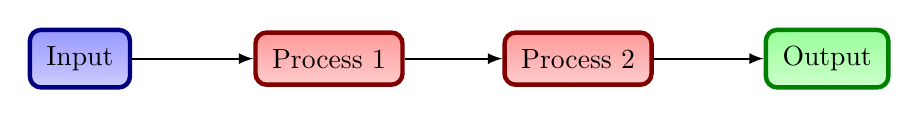
\begin{tikzpicture}[node distance=90pt]
      \tikzstyle{rect}=[line width=1.6pt,rounded corners=4pt,inner sep=6pt]
      \node[rect,top color=blue!40,bottom color=blue!20,draw=blue!50!black] (A) {Input};
      \node[rect,top color=red!40,bottom color=red!20,draw=red!50!black,right of=A] (B) {Process 1};
      \node[rect,top color=red!40,bottom color=red!20,draw=red!50!black,right of=B] (C) {Process 2};
      \node[rect,top color=green!40,bottom color=green!20,draw=green!50!black,right of=C] (D) {Output};

      \draw[-latex,thick] (A) -- (B);
      \draw[-latex,thick] (B) -- (C);
      \draw[-latex,thick] (C) -- (D);
    \end{tikzpicture}
  \end{center}
  \caption{Illustrative pipeline of the \mc process.}
  \label{fig:util:mc:pipeline}
\end{figure}
%
On the command line, we would define this as:
%
\begin{lstlisting}[style=BashInputStyle]
  MeshConvert -m process1 -m process2 input.msh output.xml
\end{lstlisting}
%
Process modules can also have parameters passed to them, that can take
arguments, or not.
%
\begin{lstlisting}[style=BashInputStyle]
  MeshConvert -m process1:p1=123:booleanparam input.msh output.xml
\end{lstlisting}
%
To list all available modules use the \inltt{-l} command line argument:
%
\begin{lstlisting}[style=BashInputStyle]
  Available classes: 
    Input: dat:
      Reads Tecplot polyhedron ascii format converted from Star CCM (.dat).
  ...
\end{lstlisting}
%
and then to see the options for a particular module, use the \inltt{-p} command
line argument:
%
\begin{lstlisting}[style=BashInputStyle]
  Options for module detect:
          vol: Tag identifying surface to process.
\end{lstlisting}
% 
\begin{notebox}
  Module names change when you use the \inltt{-p} option. Input modules should
  be preceded by \inltt{in:}, processing modules by \inltt{proc:} and output
  modules by \inltt{out:}.
\end{notebox}

\subsubsection{Input modules}

Input and output modules use file extension names to determine the correct
module to use. Not every module is capable of reading high-order information,
where it exists. The table below indicates support currently implemented.

\begin{center}
  \begin{tabularx}{\linewidth}{llcX}
    \toprule
    \textbf{Format} & \textbf{Extension} & \textbf{High-order} & \textbf{Notes}\\
    \midrule
    Gmsh & \texttt{msh} & \cmark & Only reads nodes, elements and physical groups (which are mapped to composites).\\
    Nektar & \texttt{rea} & \cmark & Reads elements, fluid boundary conditions. Most curve types are unsupported: high-order information must be defined in an accompanying .hsf file. \\
    Nektar++ & \texttt{xml} & \cmark & Fully supported. \\
    PLY & \texttt{ply} & \xmark & Reads only the ASCII format.. \\
    Semtex & \texttt{sem} & \cmark & Reads elements and boundary conditions. In order to read high-order information, run \inltt{meshpr session.sem > session.msh} and place in the same directory as the session file.\\
    Star-CCM+ & \texttt{dat} & \xmark & Reads mesh only, only support for quads and triangles (2D) and hexes, prisms, tetrahedra (3D).\\
    VTK & \texttt{vtk} & \xmark & Experimental support. Only ASCII triangular data is supported. \\
    \bottomrule
  \end{tabularx}
\end{center}

Note that you can override the module used on the command line. For example,
\texttt{Semtex} session files rarely have extensions. So for a session called
\inltt{pipe-3d} we can convert this using the syntax
%
\begin{lstlisting}[style=BashInputStyle]
MeshConvert pipe-3d:sem pipe-3d.xml
\end{lstlisting}

Typically, mesh generators allow physical surfaces and volumes to contain many
element types; for example a cube could be constructed from a mixture of hexes
and prisms. In \nekpp, a composite can only contain a single element
type. Whilst the converter will attempt to preserve the numbering of composites
from the original mesh type, sometimes a renumbering will occur when a domain
contains many element types. For example, for a domain with the tag \inltt{150}
containing quadrilaterals and triangles, the Gmsh reader will print a
notification along the lines of:

\begin{lstlisting}[style=BashInputStyle]
Multiple elements in composite detected; remapped:
- Tag 150 => 150 (Triangle), 151 (Quadrilateral)
\end{lstlisting}

The resulting file therefore has two composites of IDs \inltt{150} and
\inltt{151} respectively, containing the triangular and quadrilateral elements
of the original mesh.

\subsubsection{Output modules}

The following output formats are supported:

\begin{center}
  \begin{tabularx}{\linewidth}{llcX}
    \toprule
    \textbf{Format} & \textbf{Extension} & \textbf{High-order} & \textbf{Notes}\\
    \midrule
    Gmsh & \texttt{msh} & \cmark & Curvature output is highly experimental.\\
    Nektar++ & \texttt{xml} & \cmark & Most functionality supported. \\
    VTK & \texttt{vtk} & \xmark & Experimental. Only ASCII triangular data is supported. \\
    \bottomrule
  \end{tabularx}
\end{center}

Note that for both \gmsh and \texttt{VTK}, it is highly likely that you will
need to experiment with the source code in order to successfully generate
meshes since robustness is not guaranteed.

In the rest of these subsections, we discuss the various processing modules
available within \mc.

\subsubsection{Negative Jacobian detection}

To detect elements with negative Jacobian determinant, use the \inltt{jac}
module:
%
\begin{lstlisting}[style=BashInputStyle]
MeshConvert -m jac Mesh.xml output.xml
\end{lstlisting}
%
To get a detailed list of elements which have negative Jacobians, one may use
the \inltt{list} option:
%
\begin{lstlisting}[style=BashInputStyle]
MeshConvert -m jac:list Mesh.xml output.xml
\end{lstlisting}
%
and to extract the elements for the purposes of visualisation within the domain,
use the \inltt{extract} boolean parameter:
%
\begin{lstlisting}[style=BashInputStyle]
MeshConvert -m jac:extract Mesh.xml MeshWithNegativeElements.xml
\end{lstlisting}

\subsubsection{Spherigon patches}

Where high-order information is not available (e.g. when using meshes from
imaging software), various techniques can be used to apply a smoothing to the
high-order element. In \mc we use \emph{spherigons}, a kind of patch used in the
computer graphics community used for efficiently smoothing polygon surfaces.

Spherigons work through the use of surface normals, where in this sense
`surface' refers to the underlying geometry. If we have either the exact or
approximate surface normal at each given vertex, spherigon patches approximate
the edges connecting two vertices by arcs of a circle. In \mc we can either
approximate the surface normals from the linear elements which connect to each
vertex (this is done by default), or supply a file which gives the surface
normals.

To apply spherigon patches on two connected surfaces 11 and 12 use the following
command:
%
\begin{lstlisting}[style=BashInputStyle]
MeshConvert -m spherigon:surf=11,12 \
    MeshWithStraighEdges.xml MeshWithSpherigons.xml
\end{lstlisting}
%
If the two surfaces "11" and "12" are not connected, or connect at a sharp edge
which is $C^0$ continuous but not $C^1$ smooth, use two separate instances of
the spherigon module.
%
\begin{lstlisting}[style=BashInputStyle]
MeshConvert -m spherigon:surf=11 -m spherigon:surf=12 \
    MeshWithStraighEdges.xml MeshWithSpherigons.xml
\end{lstlisting}
%
This is to avoid the approximated surface normals being incorrect at the edge.

If you have a high-resolution mesh of the surfaces 11 and 12 in \inltt{ply}
format it can be used to improve the normal definition of the spherigons. Run:
\begin{lstlisting}[style=BashInputStyle]
MeshConvert -m spherigon:surf=11,12:usenormalfile=Surf_11-12_Mesh.ply \
    MeshWithStraighEdges.xml MeshWithSpherigons.xml 
\end{lstlisting}

This can be useful, for example, when meshing the Leading edge of an
airfoil. Starting from a linear mesh (left figure) the spherigon patches curve
the surface elements producing leading edge closer to the underlying geometry:

\begin{figure}[!htbp]
  \begin{center}
    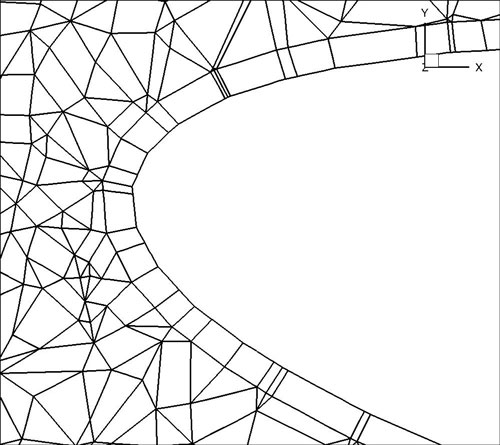
\includegraphics[width = 0.47 \textwidth]{Figures/noSphnoBL.jpg}
    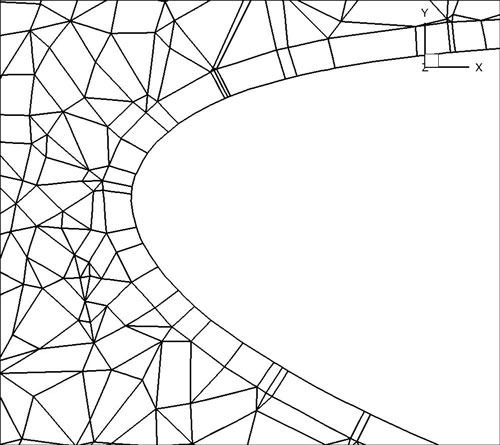
\includegraphics[width = 0.47 \textwidth]{Figures/SphnoBL.jpg}
    \caption{(a) Leading edge without spherigons, (b) Leading edge with
      spherigons}
  \end{center}
\end{figure}

\subsubsection{Periodic boundary condition alignment}

When using periodic boundary conditions, the order of the elements within the
boundary composite determines which element edges are periodic with the
corresponding boundary composite.

To counteract this issue, \mc has a periodic alignment module which attempts to
identify pairs of mutually periodic edges. Given two surfaces \inltt{surf1} and
\inltt{surf2}, which for example correspond to the physical surface IDs
specified in \gmsh, and an axis which defines the periodicity direction, the
following command attempts to reorder the composites:
%
\begin{lstlisting}[style=BashInputStyle]
MeshConvert -m peralign:surf1=11:surf2=12:dir=y \
    -m peralign:surf1=13:surf2=14:dir=z Mesh.xml Mesh_aligned.xml
\end{lstlisting}
%
Here the surfaces with IDs 11 and 12 will be aligned normal to the $y$-axis and
the surfaces 13 and 14 will be aligned normal to the $z$-axis.

Note that this command cannot perform magic -- it assumes that any given edge or
face lying on the surface is periodic with another face on the opposing surface,
that there are the same number of elements on both surfaces, and the
corresponding edge or face is the same size and shape but translated along the
appropriate axis.

In 3D, where prismatic or tetrahedral elements are connected to one or both of
the surfaces, additional logic is needed to guarantee connectivity in the XML
file. In this case we append the \inltt{orient} parameter:
%
\begin{lstlisting}[style=BashInputStyle]
MeshConvert -m peralign:surf1=11:surf2=12:dir=y:orient input.dat output.xml
\end{lstlisting}

\begin{notebox}
  One of the present shortcomings of \inltt{orient} is that it throws away all
  high-order information and works only on the linear element. This can be
  gotten around if you are just doing e.g. spherigon patches by running this
  \inltt{peralign} module before the \inltt{spherigon} module.
\end{notebox}

\subsubsection{Boundary layer splitting}

Often it is the case that one can generate a coarse boundary layer grid of a
mesh. \mc has a method for splitting prismatic and hexahedral elements into
finer elements based on the work presented in~\cite{MoHaPeSh14}
and~\cite{MoHaPeSh14b}. You must have a prismatic mesh that is $O$-type -- that
is, you can modify the boundary layer without modifying the rest of the mesh.

Given $n$ layers, and a ratio $r$ which defines the relative heights of elements
in different layers, the method works by defining a geometric progression of
points
\[
x_k = x_{k-1} + ar^k, \quad a = \frac{2(1-r)}{1 - r^{n+1}}
\]
in the standard segment $[-1,1]$. These are then projected into the coarse
elements to construct a sequence of increasingly refined elements, as depicted
in figure~\ref{fig:util:mc:split}.

\begin{figure}
  \begin{center}
    \begin{tikzpicture}
      \node[above right] at (0,0){%
        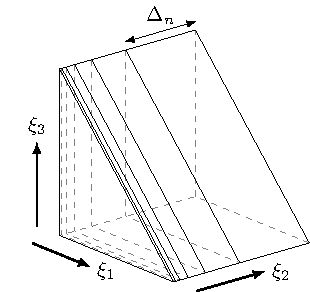
\includegraphics{utilities/Figures/stdprism_split}};
      \node[above right] at (6,0){%
        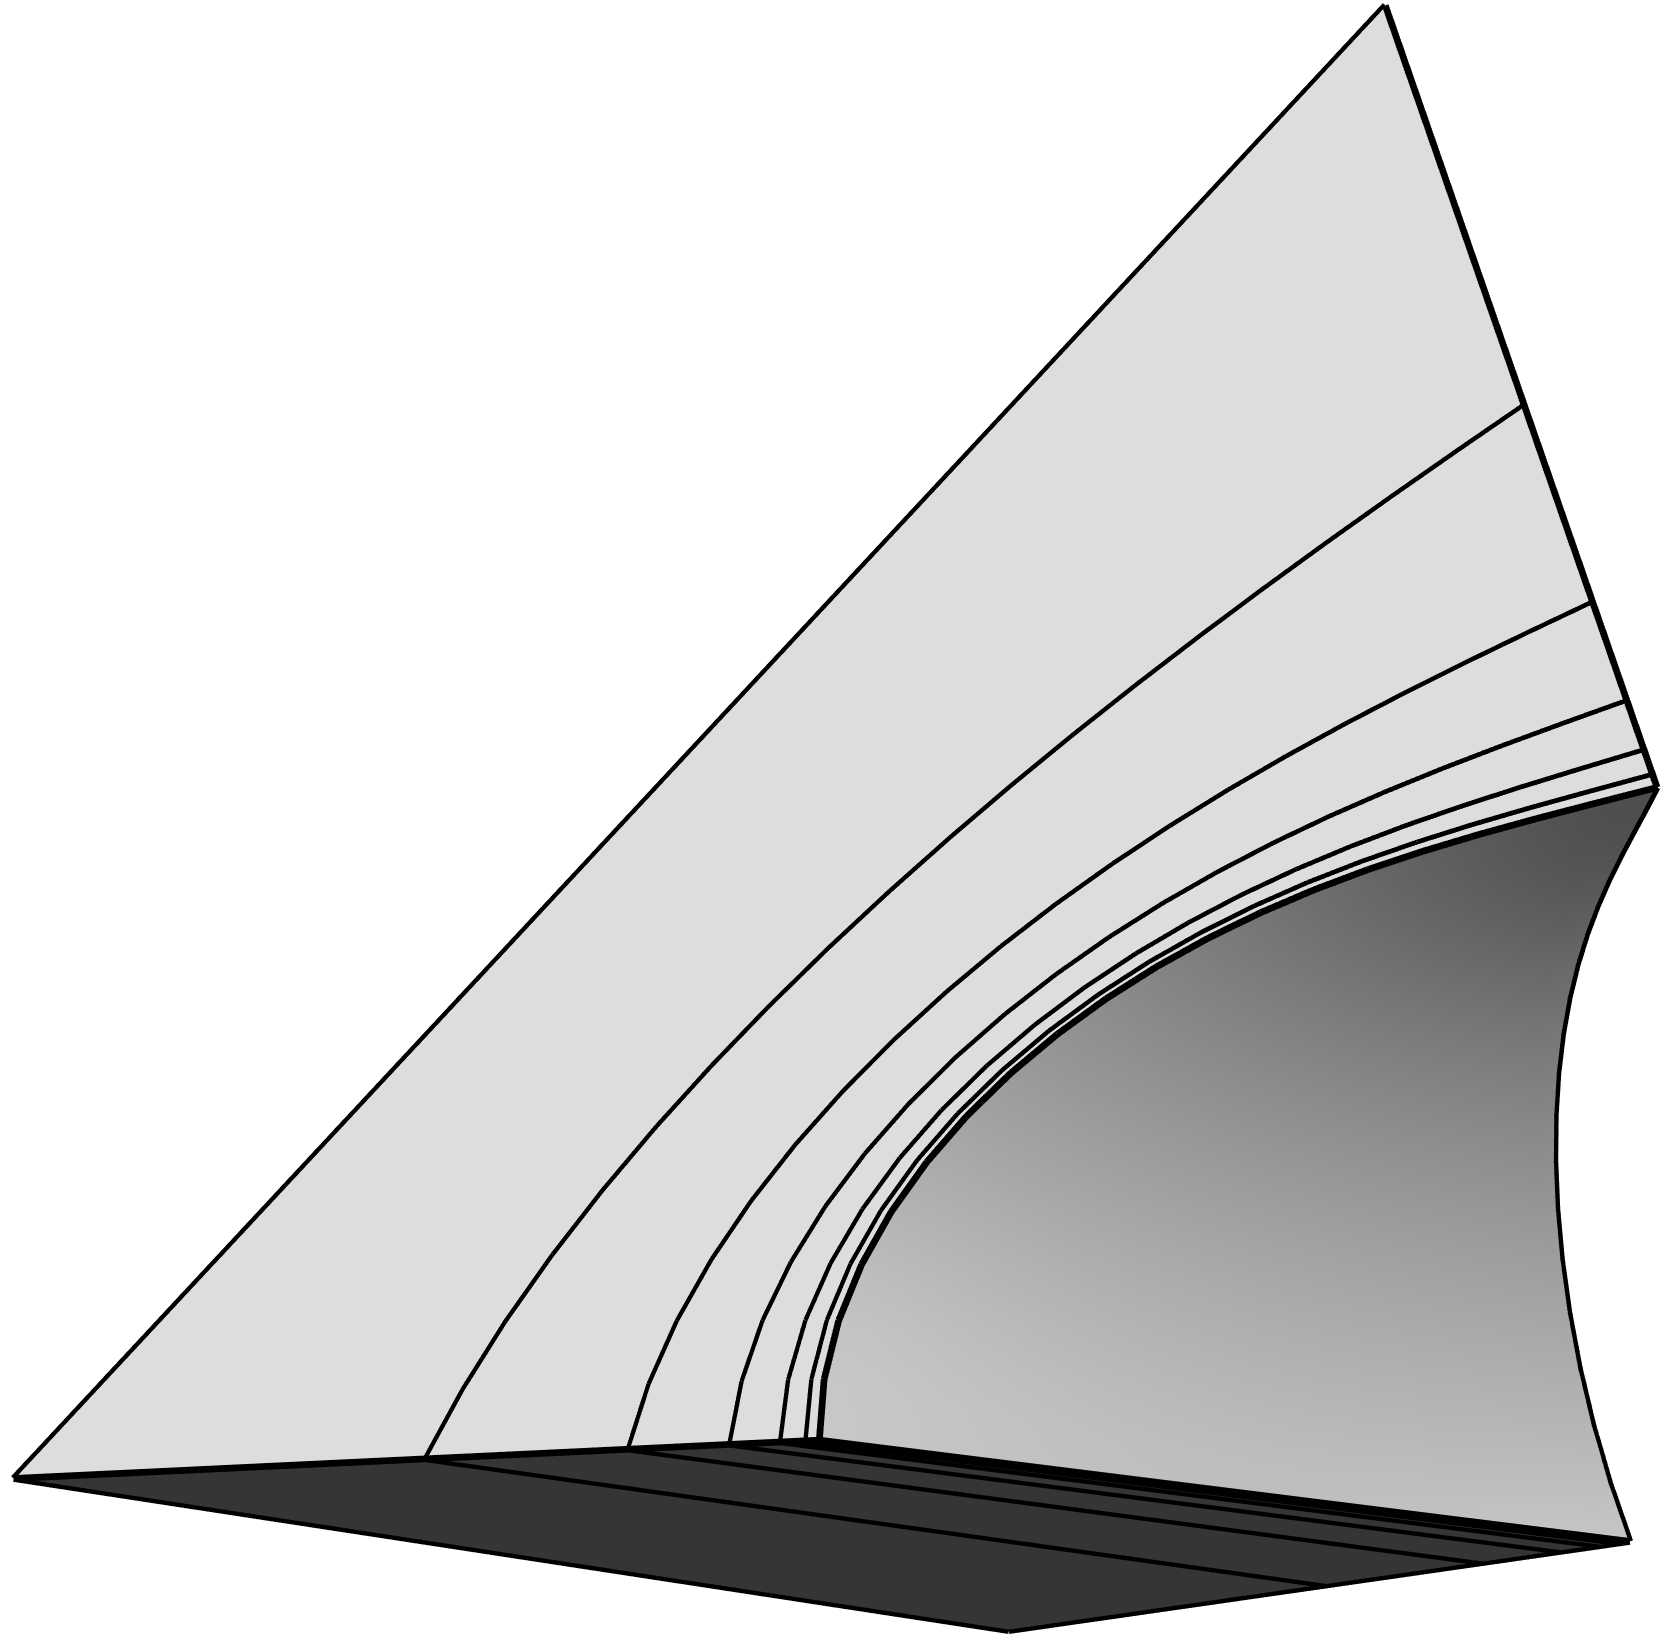
\includegraphics[width=5cm]{utilities/Figures/prism_split}};
      \draw[-latex,thick,bend left] (4.5,3.75) to[bend left]
      node[midway,above] {$\chi^e(\mathbf{\xi})$} (8.5,3.75);
    \end{tikzpicture}
  \end{center}
  \caption{Splitting $\Omega_{\text{st}}$ and applying the mapping $\chi^e$ to
    obtain a high-order layer of prisms from the macro-element.}
  \label{fig:util:mc:split}
\end{figure}

To split a prism boundary layer on surface 11 into 3 layers with a growth rate
of 2 and 7 integration points per element use the following command:
\begin{lstlisting}[style=BashInputStyle]
  MeshConvert -m bl:surf=11:layers=3:r=2:nq=7 MeshWithOnePrismLayer.xml \
        MeshWith3PrismsLayers.xml
\end{lstlisting}
%
\begin{figure}[!htbp]
  \begin{center}
    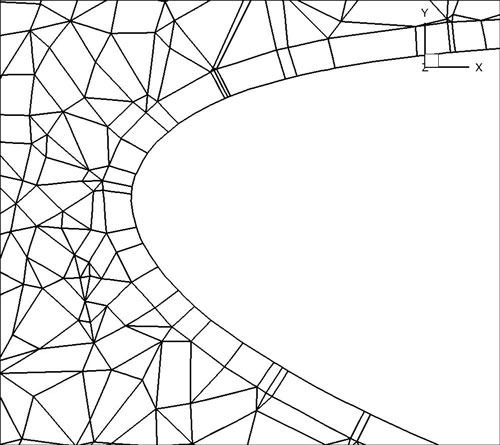
\includegraphics[width = 0.47 \textwidth]{Figures/SphnoBL.jpg}
    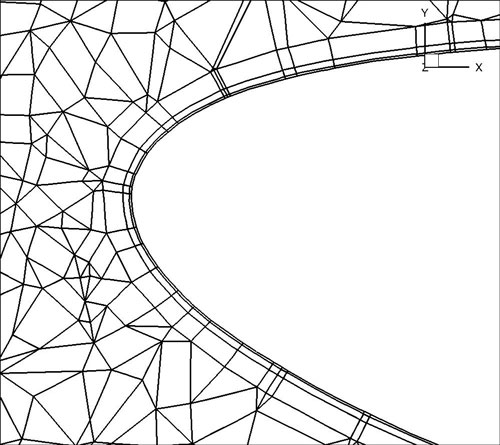
\includegraphics[width = 0.47 \textwidth]{Figures/SphBL.jpg}
    \caption{(a) LE with Spherigons but only one prism layer for resolving the
      boundary layer, (b) LE with Spherigons with 3 growing layers of prisms for
      better resolving the boundary layer.}
  \end{center}
\end{figure}

\begin{notebox}
  You can also use an expression in terms of coordinates $(x,y,z)$ for $r$ to
  make the ratio spatially varying; e.g. \inltt{r=sin(x)}. In this case the
  function should be sufficiently smooth to prevent the elements
  self-intersecting.
\end{notebox}

\subsubsection{High-order cylinder generation}

Generating accurate high-order curved geometries in \gmsh is quite challenging.
This module processes an existing linear cylindrical mesh, with axis aligned
with the $z$-coordinate axis, to generate accurate high-order curvature
information along the edges.

\begin{lstlisting}[style=BashInputStyle]
MeshConvert -m cyl:surf=2:r=1.0:N=5 LinearCylinder.xml HighOrderCylinder.xml
\end{lstlisting}

The module parameters are:

\begin{itemize}
  \item \inlsh{surf}: Surface on which to apply curvature. This should be the
  outer surface of the cylinder.
  \item \inlsh{r}: Radius of the cylinder.
  \item \inlsh{N}: Number of high-order points along each element edge.
\end{itemize}

\begin{notebox}
  The module could also be used to apply curvature along the interior of a
  hollow cylinder. However, there are no checks to ensure the resulting elements
  are not self-intersecting.
\end{notebox}

\subsubsection{Surface extraction}

Often one wants to visualise a particular surface of a 3D mesh. \mc supports
extraction of two-dimensional surfaces which can be converted using
\inltt{XmlToVtk} or similar programs for visualisation purposes, or combined
with \inltt{FieldConvert} in order to extract the value of a 3D field on a given
surface.

To extract a surface use the command:

\begin{lstlisting}[style=BashInputStyle]
  MeshConvert -m extract:surf=12,3,4 volume-mesh.xml surface-mesh.xml
\end{lstlisting}

where the integers are surface IDs to be extracted.

\subsubsection{Boundary identification}

Some mesh formats lack the ability to identify boundaries of the domain they
discretise. \mc has a rudimentary boundary identification routine for conformal
meshes, which will create a composite of edges (2D) or faces (3D) which are
connected to precisely one element. This can be done using the \inltt{detect}
module:

\begin{lstlisting}[style=BashInputStyle]
  MeshConvert -m detect volume.xml volumeWithBoundaryComposite.xml
\end{lstlisting}

\subsubsection{Scalar function curvature}

This module imposes curvature on a surface given a scalar function
$z=f(x,y)$. For example, if on surface 1 we wish to apply a surface defined by a
Gaussian $z = \exp[-(x^2+y^2)]$ using 7 quadrature points in each direction, we
may issue the command

\begin{lstlisting}[style=BashInputStyle]
  MeshConvert -m scalar:surf=1:nq=7:scalar=exp\(x*x+y*y\) mesh.xml deformed.xml
\end{lstlisting}

\begin{notebox}
  This module makes no attempt to apply the curvature to the interior of the
  domain. Elements must therefore be coarse in order to prevent
  self-intersection. If a boundary layer is required, one option is to use this
  module in combination with the splitting module described earlier.
\end{notebox}

%%% Local Variables: 
%%% mode: latex
%%% TeX-master: "../user-guide"
%%% End: 
